\documentclass{llncs}
\usepackage[colorlinks,allcolors=blue]{hyperref}
\usepackage[T1]{fontenc}
\usepackage{bookmark}
\usepackage{graphicx}
\usepackage{dirtree,array}
\usepackage{tabularray}


\graphicspath{{./images/}}


\begin{document}

    \title{Quality assurance of digital twins: An experience report in the automotive industry}

    \author{Alican Tüzün
    \and
    Georg Hackenberg
    }
    \institute{School of Engineering\\
    University of Applied Sciences Upper Austria\\
    4600 Wels, Upper Austria, Austria\\
    \email{alican.tuzuen@fh-wels.at}
    \email{georg.hackenberg@fh-wels.at}
    }
    
    \maketitle

    \begin{abstract}
        Digital twins are becoming increasingly important for the efficient and effective development 
        and operation of cyber-physical systems.
        However, digital twins are only useful if they reflect the real-world system accurately enough,
        i.e.\ their quality is high enough.
        This claim entails the question, of what the term quality in the context of digital twins means and
        how it can be measured. In this article, the authors presented their experience with the quality assurance of a digital
        twin for an assembly line in the automotive industry.
        Authors explained the preliminary definition of digital twin quality, 
        which authors derived from classical quality models for general software systems.
        Furthermore, authors described quality issues, 
        which they were able to detect in a digital twin of an assembly line in the automotive industry.
        Finally, authors concluded how to leverage their experience in different contexts 
        and how to generalize the underlying approaches.
    \end{abstract}

    \section{Introduction}\label{section:introduction}
    The notion of the digital twin, which has gained popularity in recent years, is often subject to vague and ambiguous envisions~\cite{Review1}.
    The mispresenting of this notion began with the physical twin of the Apollo 13 spacecraft. 
    The twin of Apollo 13 was merely a tangible replication of the spacecraft that has been utilized in physical simulations. 
    Even though the digital aspect was expected to be present, there wasn't~\cite{GrievesMichaelApolloMyth}.
    Another physical twin is the historic D-Day map (also known as the Big Board) in Southwick House England, 
    which was used simultaneously before and during the operation, and can be argued to be similar. 
    The board was a twin of the operation, and it included models of battalions and ships that reflected the actual 
    locations of the corresponding formations. Furthermore, synchronization was 
    implemented to give directives from the real system to control the operation 
    flow and to update the physical twin state~\cite{AMRC}.
    In contrast, a digital twin is virtual information of a possible or constructed real system, which can 
    be synchronized with a selected frequency and fidelity~\cite{Review1,Review2,digitaltwinconsortium2022}.

    The envision of a digital twin emerged from Grieves'es conceptual model, which was called mirrored spaces model in 2002~\cite{Originsofdigitaltwinconcept},
    and later referenced in a 2005 journal article~\cite{2005ArticleGrievesMichael}. 
    Furthermore, he introduced the information mirroring model, which was his ideal form of product lifecycle management
    at that time with only one goal. The goal was to gather as much relevant and useful information about the real system and leverage that information to trade the required energy, time, 
    and material sources for the system operations.
    Initially, this model had four main parts. The real system, virtual system, connection between the real and virtual system and virtual simulations~\cite{GrievesPLMBook}. 
    Later, Grieves removed the latter, to simplify the model~\cite{Originsofdigitaltwinconcept}. Lastly, after co-authoring with Vicker in 2010, 
    Grieves decided to use the NASA-invented `Digital Twin' word, instead of the information mirroring model~\cite{Originsofdigitaltwinconcept}.

    In recent years, there is evidence that digital twins play a crucial role in the manufacturing industries, life sciences, healthcare, infrastructure and smart cities~\cite{Review2}.
    For example, a digital wind farm from General Electric is a good illustration of how building a digital twin helped to design a better turbine, 
    which was used to collect and analyze the data from the real system for making the process of the real system more efficient~\cite{GeneralElectricWindTurbine}. 
    Another fascinating example of the use of digital twins is Philips' virtual heart model. The twin of the heart evolves with the data generated by ultrasonic sensors to calculate 
    how well the real heart is pumping the blood. This information can be used to predict a potential heart failure, allowing for early intervention and potentially life-saving treatment~\cite{PhilipsHearth}. 
    Lastly, FELICE is another interesting example of a digital twin application in manufacturing. In the project, twin models of machines/equipment and 
    agents are utilized to support real-time decision-making and to conduct what-if analysis and experiments~\cite{FELICE}.

    The previous studies predominantly focused on the design and implementation of digital twins~\cite{Review1,Review2}. 
    However, a crucial aspect that remains unclear is how to achieve quality in these highly intricate and evolvable systems. 
    Therefore, ascertaining the requisite level of quality of a digital twin is an arduous undertaking that requires further research.

    This paper aims not only to review the digital twin artifacts utilized in the FELICE project and evaluate the quality issues associated with them~\cite{FELICE},  
    but also, targets to enhance the scientific understanding of the quality of digital twins. The artifacts analyzed in this study include process videos showing the current assembly procedure, 
    a scope definition, a requirements specification, a general and operational conceptual model, and a discrete event simulation module. 
    To evaluate these artifacts, we considered five crucial quality attributes: correctness, completeness, fidelity, efficiency, and evolvability.
    
    \section{Related Work on Quality}
    The notion of quality is defined in many forms in the literature. Some scholars defined quality as conformance to specifications and
    requirements~\cite{ProductConformanceCostGilmore,LevittTheodoreProduction-LineApproach,QualityisFree}, while others saw it as a value~\cite{QualityandCompetitionanEssayinEconomicTheory} or the 
    fitness for use~\cite{Juran1974}which evolved to fitness for purpose later~\cite{Juran2010},  
    or an abstain of loss~\cite{GenichiTaguchi}, and meeting or exceeding customer expectations~\cite{Groenrossstrategicmanagementandmarketing}. 
    Even the ISO9000 standard defines the quality differently, which is an inherent characteristic of the entity~\cite{ISO9000}. 
    These definitions endeavors to provide an universal understanding of quality and assess it subsequently. However, 
    they come with some strengths and weaknesses. For example, conforming to the requirements and specifications can be useful for assessing the quality of the system but may not always reflect the needs of the stakeholders,
    hence the quality of the system depends on how accurately these requirements were set~\cite{IEE7302014}. 
    
    The first serious discussions of subcategorization of quality trace back to the beginning of the 20th century with the emergence of product-focused quality management practices in manufacturing~\cite{HistoryofControlEngineering}.
    Later on, with the development of new technologies, subcategorization of quality was evolved and extended to other areas, such as software, which appeared in the 1970s~\cite{ThePsychologyofComputerProgramming}.
    With this emergence, assessing the software quality became inevitable and as a result, a considerable amount of software quality models and characteristics have been established~\cite{SoftwareQualityModels,Charecteristicsofsoftwarequality,AnActivityBasedQualityModelforMaintainability}.
    As an example, ISO/IEC:25010 has standardized eight software quality characteristics, including functional suitability, performance efficiency, compatibility, usability, reliability, security, maintainability, 
    and portability, to determine software quality~\cite{ISO/IEC:25010}.
    
    It was not until the late 1950s that another important subcategory for the context of this paper `computer simulation quality' 
    was considered~\cite{SomeProblemsofDigitalSystemsSimulation}. Surprisingly, R. W. Conway et al.identified several potential problems with computer simulation systems in this era, which are still relevant today.  
    To find and evaluate these problems, validation and verification techniques have emerged~\cite{StewartSimulation,VerificationValidationSergent,OsmanBalci}. 
    Validation is the process of evaluating the simulation quality in comparison to the real system from the perspective of its intended applications. 
    On the other hand, verification is a procedure to evaluate the implementation of the simulation model and its associated data concerning the conceptual description and specifications of 
    the model developer~\cite{StewartSimulation,VerificationValidationSergent}. These techniques are broadly categorized into six areas: informal, static, dynamic, symbolic, constraint, 
    and formal techniques~\cite{balcicategories,balcitechniques}. Formal techniques involve mathematical formality, 
    whereas informal techniques rely on human intervention and reasoning. Although mathematical techniques are more precise, informal techniques are more commonly used~\cite{balcicategories}.

    \subsection{Digital Twin Quality}
    To analyze the state of the digital twin quality, a literature analysis was executed. 
    The analysis especially focused on how the digital twin quality is mentioned and assessed within the academic dissertations. Therefore, various tools, such as Scopus and Google Scholar were 
    used to perform an extensive literature analysis on digital twin publications. However, due to the vast amount of available literature, the scope of the research was narrowed down, resulting in the identification of 
    150 dissertations linked to digital twin quality, verification and validation. After a thorough review of these, only 17 were considered relevant for this paper, and as a result following findings were revealed.
  
    First, He Zhang et al. developed a consistency evaluation approach for digital twin models, which can be used to assess their quality. 
    The authors also discuss essential concepts, such as consistency between real and virtual systems and ultra-fidelity models~\cite{ZHANGEVALUATIONMETHOD}. 

    In yet another insightful article, He Zhang et al. introduced the updating method for digital twin models.
    Once more, the accuracy and coherence of the model concepts were addressed~\cite{ZHANGUPDATEMETHOD}.

    Furthermore, Selch et al. presented a machine-learning approach based on Bayesian networks to track the quality of the digital twin. 
    The unique aspect of this study is that the authors determined the contributions of subsystems to forecast the overall quality of the digital twin, 
    rather than just analyzing it as a single system. The digital couplings, which are linkages between the subsystems, are also identified as a source of extra uncertainty. 
    However, since only one digital twin has been used in practice, multiple subsystem digital twins have not been validated~\cite{QualityMonitoringofCoupledDigitalTwins}.

    Additionally, the stability of digital twin models was assessed by another study using the Kolmogorov-Smirnov statistical test, 
    which measures the degree of similarity between the probability distribution of the model's predictions and the distribution of the actual data~\cite{RadarDigitalTwin}.

    Edward Y. Hua et al. identify five open problems with digital twin model validation, including modeling realism, data uncertainty, system dynamics, use-case alignment, and reporting invalid modes.
    To address these challenges, the authors propose a digital-twin model validation framework. The paper also highlights three areas for future research, 
    including uncertainty and sensitivity analysis, model validation of system-of-systems, and combining expert knowledge and collected data ~\cite{ValidationofDigitalTwins}. 

    Finally, Shotaro Hamato et al. demonstrated successful real-time anomaly detection using the Unscented Kalman Filter with the digital twin model. 
    However, determining the appropriate threshold for anomaly detection remains problematic~\cite{JapeneseKalmanFilterCorrectness}.

    These dissertations provide valuable insights into various aspects of digital twin quality assessment, including model consistency, stability, and validation, as well as machine learning-based approaches and real-time anomaly detection. 
    However, the identified open problems, including modeling realism, data uncertainty, system dynamics, use-case alignment, and reporting invalid modes, call for further research in the field to improve the quality and reliability of digital twins. Moreover, 
    the lack of well-defined quality parameters for digital twins puts forward a significant challenge in ensuring their quality, which necessitates the development of appropriate quality metrics and standards for digital twins.
    
    \section{Method}
    The form of FELICE's digital twin was the digital twin instance\cite{GrievesVickers2017}, 
    which implies that the real system was already constructed. 
    It is important to note that, for the sake of convenience, 
    the authors utilized the term `Digital Twin' in the subsequent chapters instead of `digital twin instance'.

    Moreover, since the digital twin was still in the design phase, 
    the methodology of assessing its quality consists of several key steps,
    including identification of the artifacts, manual reviews of these artifacts, 
    mapping quality attributes to the identified findings, an evaluation of the artifact quality, and ultimately, 
    an evaluation of the digital twin's overall quality.
    \subsection{Artifacts}\label{section:Artifacts}
    The current stage of review encompassed five key artifacts,
    including process videos displaying the current assembly procedure without an adaptive workstation and cobot,
    a scope definition outlining the objects on the shop floor requiring tracking or twinning, a requirements 
    specification summarizing functional and non-functional requirements for the digital twin, a general and an operational 
    conceptual model elucidating the high-level structure of the assembly procedure, 
    and a discrete event simulation module that implements the structures prescribed by the conceptual models.

    \textbf{Process Videos} have been utilized to explain the manual assembly procedures performed at each of the three workstations. From the three videos initially provided by the project partner,  
    the sequence of assembly steps was extracted at least for one product variant. The tools and the parts needed for each assembly operation were observed. Additionally, the approximate duration of each assembly step 
    was estimated, and some ergonomic characteristics of each operation were derived. 
    The derivable ergonomic characteristics mainly included the poses and motions performed by the operators.

    \textbf{Scope Definition} was determined using a methodology based on hierarchical task analysis and process videos provided by the project partner, which aids in better understanding the context and focus of the digital twin.
    This resulted in a scope definition that identified entities to be twinned, entities to be tracked, and important areas in the scene. 
    Entities to be twinned needed to be represented accurately in the simulation models, including their position, pose, speed, fatigue, and other state variables. 
    Entities to be tracked, on the other hand, only required position information. The scope definition was based on a floor plan of the production facility, with the three workstations marked as gray rectangles. 
    The human workers, cobot, and adaptive workstation were identified as entities to be twinned, and therefore required accurate representation, 
    monitoring, and simulation. Other entities, such as an AGV, carts with doors, and screwdrivers used for assembly operations, were designated as entities to be tracked.

    \textbf{Requirements Specification} for the digital twin was defined with a unique ID, a natural language description, an origin, a category, a priority, and a rationale. The ID was used as a reference point for other project artifacts, while the specification described the requirement in a way that allowed for testing of the digital twin implementation. The origin of the requirement was noted to identify the project partner responsible for its creation.
     The category is distinguished between functional and non-functional requirements, as well as constraints and standards. The priority of each requirement was classified into four levels 
    (must-, should-, could-, and would-have) to help prioritize development efforts. 
    Finally, the rationale provided a clear explanation for each requirement's implication in the specification.

    \textbf{Conceptual Model} was comprised of two parts: a general conceptual model and an operational conceptual model. 
    Both models described the assembly line processes however the operational conceptual model focused on the specific steps of the assembly process, while the general conceptual model focused on higher-level processes and workflows.
    The general conceptual model was represented using a general flow chart notation which distinguishes a root node, activity nodes, and decision nodes.
    The operational conceptual model consisted of three spreadsheets, each displaying the sequence of assembly operations performed at one workstation. 
    The assembly operations were divided into macro- and micro-operations, with each macro-operation referring 
    to one part of the final product being assembled, and the micro-operations referring to the individual steps needed to complete the respective macro-operation.

    \textbf{Discrete Event Simulation Model} consisted of seven sections, including two animation sections, two input sections, one output section, one process logic section, and a database section. 
    The animation sections provided a two-dimensional and a three-dimensional representation of the system, 
    which aided in understanding the simulation and debugging purposes. The input sections allowed for the management of inputs to the simulation model, and the output section displayed summary performance indicators about the simulation run. 
    The process logic section contained the process building blocks, such as queues and assembly operations. Lastly, the database section provided an interface to data sources and sinks.
    
    \subsection{Manual Artifact Reviews}
    During the initial stages of the project, when the target system was not yet available,
    there was a lack of observable data about system behavior that could be utilized for validation. 
    Instead, informal and potentially incomplete, inconsistent, or incorrect system descriptions had to be relied upon. 
    Therefore, manual reviews were deemed the most suitable tool to account for the characteristics of this situation.
    The manual review included audits, inspections, reviews, structural analysis and walkthroughs 
    with the project partners which was inspired by Balci's manual review works~\cite{balcitechniques}. 
    
    \subsection{Digital Twin Quality Attributes}\label{section:Digital Twin Quality Attributes}
    To identify the digital twin quality attributes, the following standards, including ISO/IEC:25010, IEE730-2014, ISO9000, and ISO9001, 
    as well as the Oxford dictionary was consulted to 
    synthesize our findings\cite{ISO9000,ISO90012015,ISO/IEC:25010,IEE7302014,OxfordDictionary}.

    \textbf{Correctness} is a  derived word from the adjective \textit{correct}, which means that the entity is error-free regarding fact or truth. 
    In the context of the digital twins, the fact or truth is the real system hence, \textit{correctness} is a grade of quality, 
    that indicates an error between the real system and a digital twin system (Figure~\ref{fig:CorrectnessAndCompleteness}).
    Meanwhile, the quality of being \textit{correct} is measured by the metric accuracy~\cite{OxfordDictionary}. 

    \begin{figure}[htbp]
        \centering
        \includegraphics[width = 1\textwidth]{CorrectnessandCompleteness.png}
        \caption{Incorrect (a) and incomplete (b) status has been demonstrated with a simplified finite state machine. Incorrectness can be observed in the behavior 
        of the machine after 2 state transitions. Incompleteness, on the other hand, can be observed in the missing state. It should be noted that, even though the second state machine is missing a 
        component, it shows the right behavior, hence it is correct.}\label{fig:CorrectnessAndCompleteness}
    \end{figure}

    \textbf{Completeness} is a derived word from the word  \textit{complete}, which can be described as an adjective, attribute, or verb~\cite{OxfordDictionary}. 
    The adjectival form used in the study denotes \textit{complete} as a state of having all the necessary or appropriate parts according to the real system 
    (Figure~\ref{fig:CorrectnessAndCompleteness}). Additionally, subaspects of completeness, which are \textit{incompleteness} and \textit{overcompleteness} 
    were inspected but identified as a completeness issue.  

    \textbf{Fidelity} refers to the degree of exactness with which the real system is copied and represented. 
    Low fidelity indicates a simplified representation, 
    while high fidelity refers to an accurate and detailed representation of the real system~\cite{Review2} (Figure~\ref{fig:EfficiencyandFidelity}). 
    The concept of fidelity has garnered significant attention in recent
    years and continues to be an important focus in Digital Twin research~\cite{Review2,Review1}.

    \textbf{Efficiency} refers to the quality of being efficient~\cite{OxfordDictionary}. 
    Therefore, \textit{efficiency} is achieving maximum productivity with minimum wasted resources (Figure~\ref{fig:EfficiencyandFidelity}). 
    It is worth mentioning that the concept of \textit{efficiency} is tightly coupled with the notion of productivity, 
    although \textit{efficiency} differs from the latter's definition, which is defined as the capability to produce large amounts of goods~\cite{OxfordDictionary}.  
    For example, time efficiency indicates that,  with less amount of time as an input, more output with the minimum waste during the process is desired (Figure~\ref{fig:EfficiencyandFidelity}).
    \begin{figure}[htbp]
        \centering
        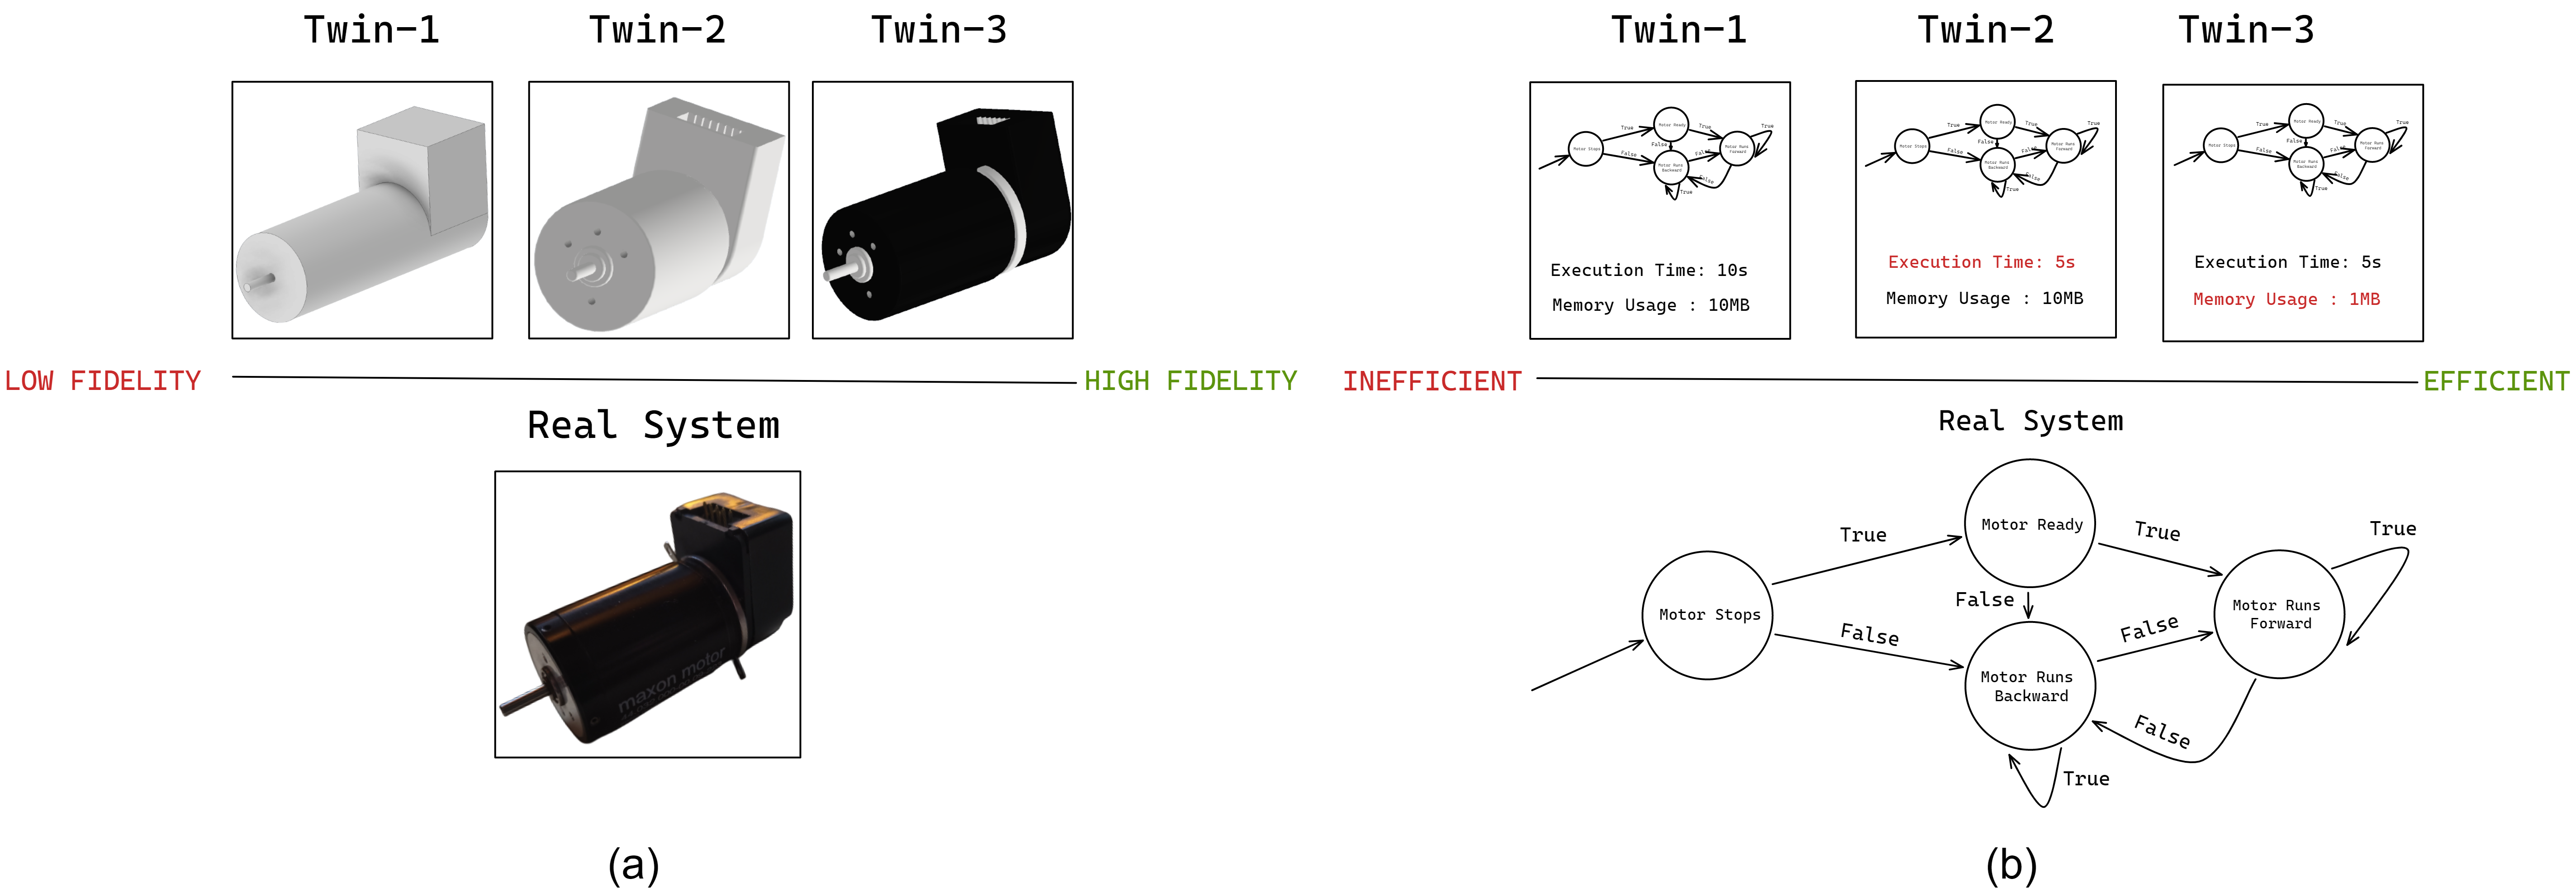
\includegraphics[width = 0.9\textwidth]{Efficiency and Fidelity.png}
        \caption{Fidelity and Efficiency levels have been demonstrated with simplified CAD drawings. For the assessment of 
        Efficiency, quantitative metrics, rendering time, and model size have been utilized.}~\label{fig:EfficiencyandFidelity}
    \end{figure}

    \textbf{Evolvability} is a system's capability to enhance its suitability to its environment through alterations to both its internal and functional 
    structure\cite{MobusSystemTheory}. Another term to describe the response to changes in the environment is adaptability.
    However, this concept differs from \textit{evolvability} in that it only affects a system's internal or functional structure temporarily. 
    For instance, a digital twin, which is an evolvable virtual system, can be designed to be more flexible and scalable, 
    allowing for easy updates and the addition of new features\cite{ZHANGUPDATEMETHOD}. 
    Furthermore, the evolvability of the digital twin was assessed based on the quantity of effort, which is a necessary resource to initiate transformation
    within the system (Figure~\ref{fig:Evolvability}). 
    \begin{figure}[htbp]
        \centering
        \includegraphics[width = 0.9\textwidth]{Evolvability.png}
        \caption{Figure represents the demonstration of evolvability with the comparison between the first state machine(represented in black), and the evolved state machine(represented in green). The required effort
        to evolve from the black state machine to the green state machine could be evaluated as \textit{Evolvability}.}~\label{fig:Evolvability}
    \end{figure}
    \subsection{Mapping Digital Twin Attributes to Manual Review Results}
    To evaluate the quality of the artifact, the issues were mapped to digital twin attributes. 
    To begin this process, the findings were collected from the manual review, followed by an inspection of the findings to determine which digital twin qualities were absent. 
    Finally, the findings were mapped to the relevant missing quality attribute(s) and submitted for artifact quality evaluation (Figure~\ref{fig:Method}).
    \subsection{Artifact Quality Evaluation}
    To evaluate the quality of the digital twin artifacts, the mapped findings were scrutinized and evaluated. 
    The process started by identifying which quality attribute(s) were mapped. 
    Once identified, the missing attribute(s) was incremented by 1 to determine the total quality of missing attributes of the artifact(Figure~\ref{fig:Method}).
    \begin{figure}[htbp]
        \centering
        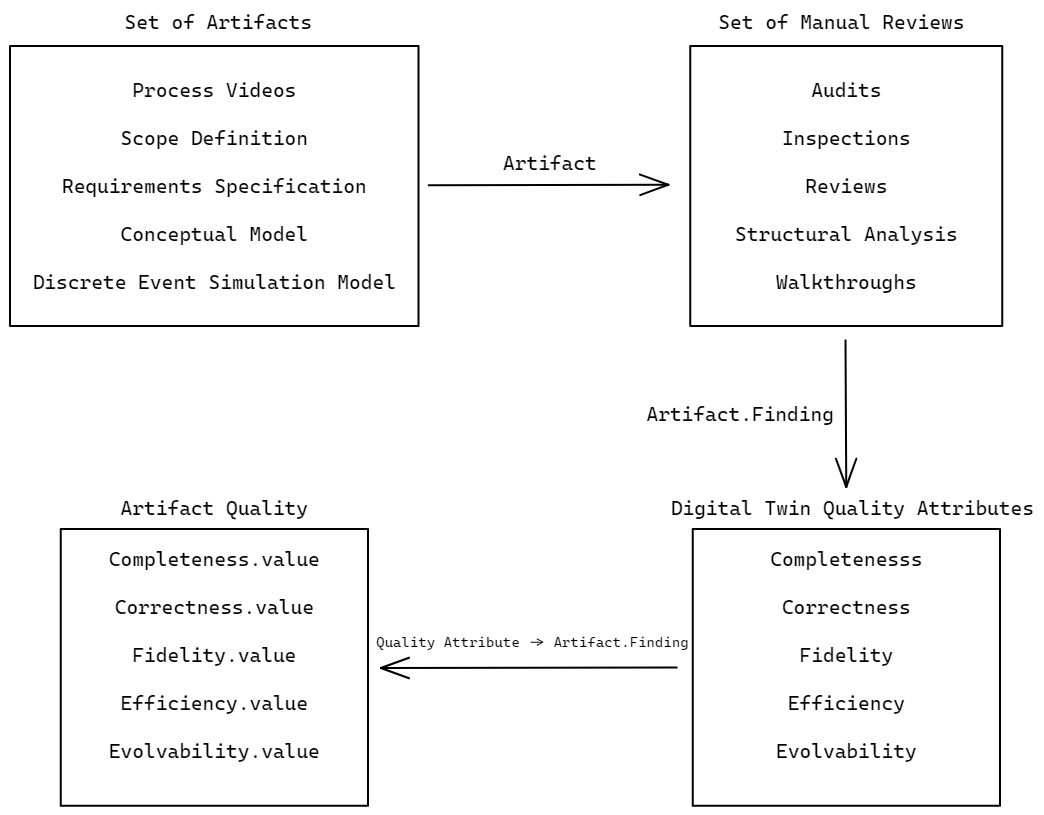
\includegraphics[width = 0.8\textwidth]{RequirementSpecifications.png}
        \caption{Method for the evaluation of the digital twin artifact quality: `Artifact.finding' indicates that the finding belongs to the artifact, while `->' indicates mapping}\label{fig:Method}
    \end{figure}
    \subsection{Digital Twin Quality Evaluation}
    To determine the quality of the digital twin, 
    the values obtained from evaluating each artifact's quality were collected and summed. 
    Furthermore, the value of the sum was assigned to the related digital twin quality attribute. 
    As a result, the digital twin quality was demonstrated with quality attribute values (Figure~\ref{fig:MethodforDigitalTwinQuality}).
    \begin{figure}[htbp]
        \centering
        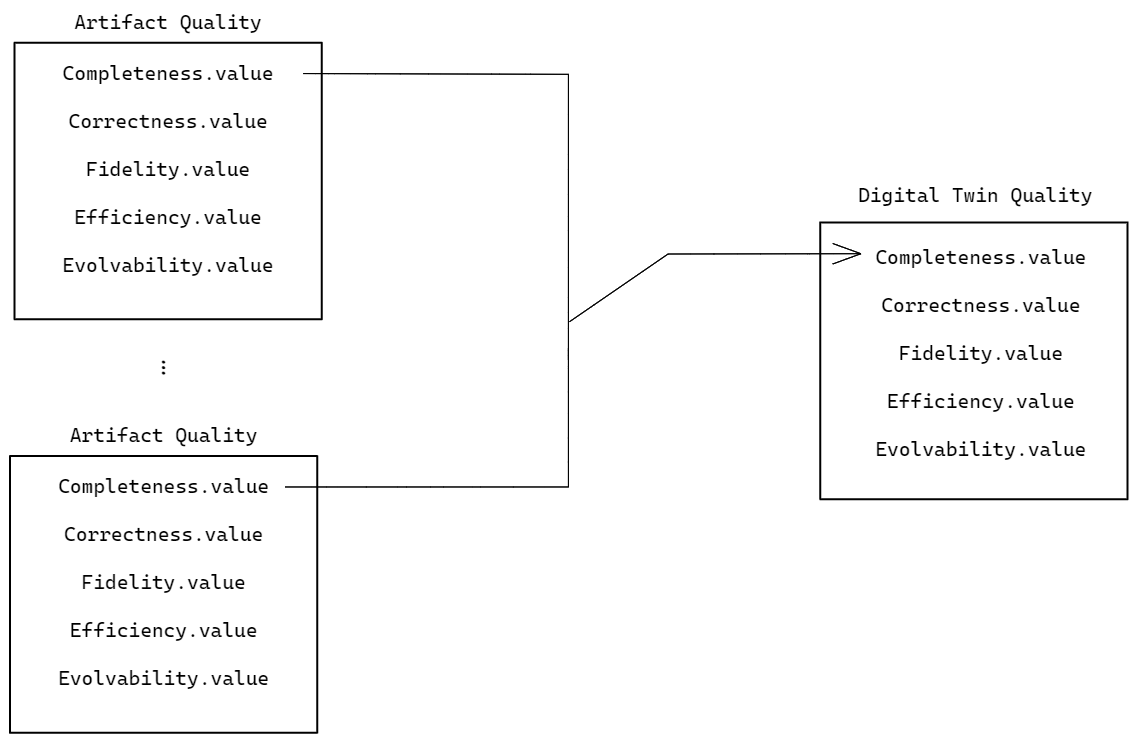
\includegraphics[width = 0.8\textwidth]{DigitalTwinQuality.png}
            \caption{Method for the evaluation of the digital twin quality}\label{fig:MethodforDigitalTwinQuality}
    \end{figure}
    \section{Results}
    First, to assess digital twin quality, manual reviews for each artifact were conducted (Figure~\ref{fig:QualityInspectonResultsWithArtifacts}). 
    As a result, a total of twenty-one quality related issues were identified, listed, and finally mapped to the digital twin quality attributes (Table~\ref{tab:Table1}) (Figure~\ref{fig:QualityInspectonResultsWithArtifacts}).
    The mapping process revealed that a total of thirty-eight digital twin quality attributes were lacking in the artifacts (Figure~\ref{fig:QualityInspectonResultsWithArtifacts}).  
    Specifically, 23\% of the quality issues of the digital twin were related to correctness, which indicates an error between the real- and digital twin system. Furthermore, 36\%  were related 
    to completeness, proving that some necessary or appropriate parts were missing.
    Moreover, 8\%  were related to fidelity, indicating a lack of detail. 
    In addition, 5\%  were related to efficiency, indicating poor performance or excessive resource usage.
    And finally, 28\% were related to evolvability, indicating that the system was unresponsive 
    to the environment and was not flexible or scalable.
    \subsection{Example Findings}  
    Two examples (Finding 12, Finding 18) are given to the reader to illustrate 
    the results of the manual review as well as the mapping to the digital twin quality attributes. 
    \subsubsection{Conceptual Model-Finding 12:}
    The duration of the micro-operations in the conceptual model was calculated using a simple calculation 
    scheme based on the duration of the corresponding macro-operations,
     which were well-known from a prior well-conducted study. 
    However, relying on estimated, 
    simplified calculations for the micro-operation durations,
    suggests that the digital twin conceptual model suffers from issues of correctness and completeness (Table~\ref{tab:Table1}). 
    \subsubsection{Simulation Model-Finding 18:}
        The discrete event simulation model enforced a strictly sequential execution of micro-operations,
        which precludes the support of parallel execution. 
        However, machine-human collaboration on a task, needs a parallel execution, especially when the cobot overtakes certain micro-operations. 
        Thus, the exclusion of parallel executions indicates that the simulation model was incomplete,
        at the same time, using the wrong type of execution highlights its inaccuracies (Table~\ref{tab:Table1}).
    \begin{figure}[htbp]
            \centering
            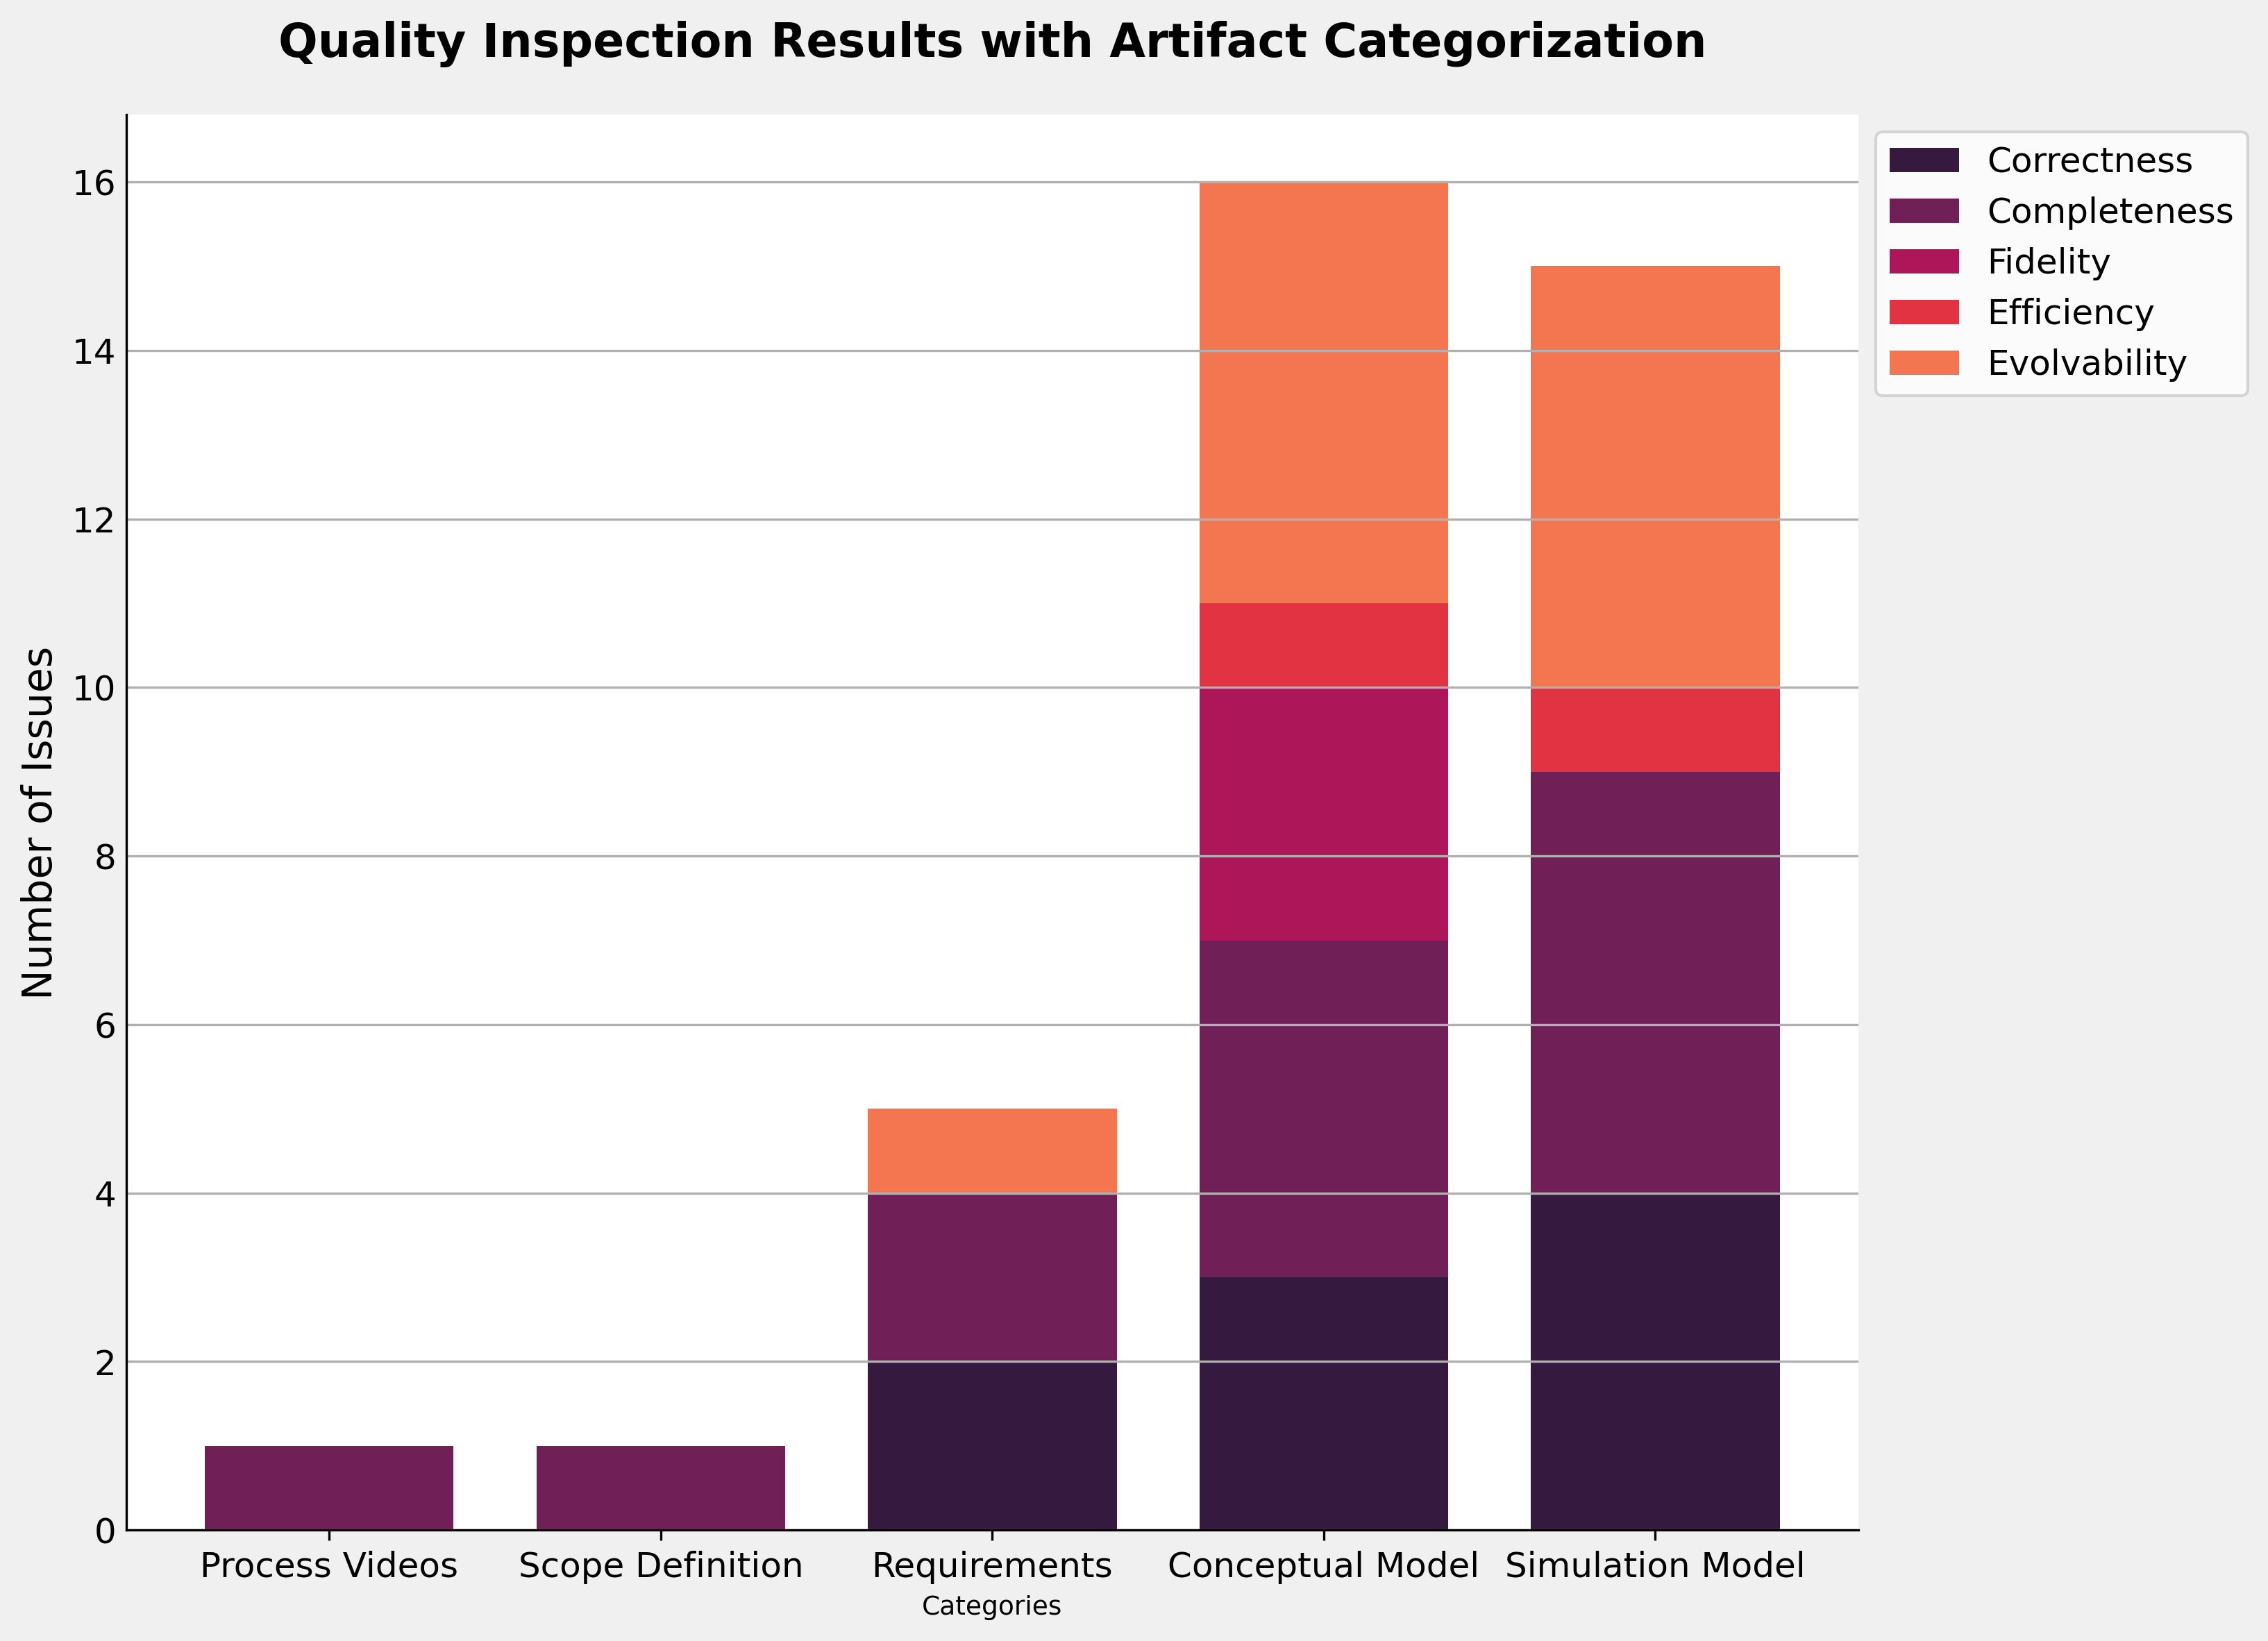
\includegraphics[scale = 0.35]{quality_inspection_results_with_artifacts.png}
            \caption{Quality Inspection Results Categorized with Artifacts: X-Axis represents artifacts in section \ref{section:Artifacts}, 
            Y-Axis represents the number of missing quality attributes found for each artifact, 
            and lastly, each digital twin quality attribute is shown by the colors.}\label{fig:QualityInspectonResultsWithArtifacts}
    \end{figure}
    \begin{table}[h!]
        \begin{center}
        \caption{Mapping of digital twin attributes to the results of the 
        manual reviews: Cases where an attribute is mapped, were marked by `X'.}\label{tab:Table1}
        \scalebox{0.75}{
            \begin{tabular}{llllll}
                \multicolumn{1}{c}{\textbf{Findings}} & \multicolumn{1}{c} {\textbf{Correctness}} & \multicolumn{1}{c}{\textbf{Completeness}} 
                & \multicolumn{1}{c}{\textbf{Fidelity}} & \multicolumn{1}{c}{\textbf{Efficiency}} & \multicolumn{1}{c}{\textbf{Evolvability}} \\
                \hline
                \begin{minipage}{4cm}\dirtree{%
                    .1 Artifacts.
                    .2 Process Videos.
                    .3 Finding 1.
                    .2 Scope Definition.
                    .3 Finding 2.
                    .2 Requirement Specs.
                    .3 Finding 3.
                    .3 Finding 4.
                    .3 Finding 5.
                    .3 Finding 6.
                    .2 Conceptual Model.
                    .3 Finding 7.
                    .3 Finding 8.
                    .3 Finding 9.
                    .3 Finding 10.
                    .3 Finding 11.
                    .3 Finding 12.
                    .2 Simulation Model.
                    .3 Finding 13.
                    .3 Finding 14.
                    .3 Finding 15.
                    .3 Finding 16.
                    .3 Finding 17.
                    .3 Finding 18.
                    .3 Finding 19.
                    .3 Finding 20.
                    .3 Finding 21.
                }\end{minipage}
                &
                \DTsetlength{0pt}{0pt}{0pt}{0pt}{0pt}
                \begin{minipage}{2cm}\dirtree{%
                    .1 \empty.
                    .2 \empty.
                    .3 ~~~~~0.
                    .2 \empty.
                    .3 ~~~~~0.
                    .2 \empty.
                    .3 ~~~~~X.
                    .3 ~~~~~X.
                    .3 ~~~~~0.
                    .3 ~~~~~0.
                    .2 \empty.
                    .3 ~~~~~X.
                    .3 ~~~~~0.
                    .3 ~~~~~0.
                    .3 ~~~~~X.
                    .3 ~~~~~0.
                    .3 ~~~~~X.
                    .2 \empty.
                    .3 ~~~~~0.
                    .3 ~~~~~X.
                    .3 ~~~~~X.
                    .3 ~~~~~0.
                    .3 ~~~~~X.
                    .3 ~~~~~0.
                    .3 ~~~~~0.
                    .3 ~~~~~0.
                    .3 ~~~~~0.
                }\end{minipage}
                &
                \DTsetlength{0pt}{0pt}{0pt}{0pt}{0pt}
                \begin{minipage}{2cm}\dirtree{%
                    .1 \empty.
                    .2 \empty.
                    .3 ~~~~~X.
                    .2 \empty.
                    .3 ~~~~~X.
                    .2 \empty.
                    .3 ~~~~~X.
                    .3 ~~~~~X.
                    .3 ~~~~~0.
                    .3 ~~~~~X.
                    .2 \empty.
                    .3 ~~~~~X.
                    .3 ~~~~~X.
                    .3 ~~~~~0.
                    .3 ~~~~~X.
                    .3 ~~~~~0.
                    .3 ~~~~~X.
                    .2 \empty.
                    .3 ~~~~~X.
                    .3 ~~~~~X.
                    .3 ~~~~~X.
                    .3 ~~~~~0.
                    .3 ~~~~~X.
                    .3 ~~~~~X.
                    .3 ~~~~~X.
                    .3 ~~~~~0.
                    .3 ~~~~~0.
                }\end{minipage}
                &
                \DTsetlength{0pt}{0pt}{0pt}{0pt}{0pt}
                \begin{minipage}{2cm}\dirtree{%
                    .1 \empty.
                    .2 \empty.
                    .3 ~~~~~0.
                    .2 \empty.
                    .3 ~~~~~0.
                    .2 \empty.
                    .3 ~~~~~0.
                    .3 ~~~~~0.
                    .3 ~~~~~0.
                    .3 ~~~~~0.
                    .2 \empty.
                    .3 ~~~~~X.
                    .3 ~~~~~X.
                    .3 ~~~~~0.
                    .3 ~~~~~X.
                    .3 ~~~~~0.
                    .3 ~~~~~0.
                    .2 \empty.
                    .3 ~~~~~0.
                    .3 ~~~~~0.
                    .3 ~~~~~0.
                    .3 ~~~~~0.
                    .3 ~~~~~0.
                    .3 ~~~~~0.
                    .3 ~~~~~0.
                    .3 ~~~~~0.
                    .3 ~~~~~0.
                }\end{minipage}
                &
                \DTsetlength{0pt}{0pt}{0pt}{0pt}{0pt}
                \begin{minipage}{2cm}\dirtree{%
                    .1 \empty.
                    .2 \empty.
                    .3 ~~~~~0.
                    .2 \empty.
                    .3 ~~~~~0.
                    .2 \empty.
                    .3 ~~~~~0.
                    .3 ~~~~~0.
                    .3 ~~~~~0.
                    .3 ~~~~~0.
                    .2 \empty.
                    .3 ~~~~~X.
                    .3 ~~~~~0.
                    .3 ~~~~~0.
                    .3 ~~~~~0.
                    .3 ~~~~~0.
                    .3 ~~~~~0.
                    .2 \empty.
                    .3 ~~~~~0.
                    .3 ~~~~~0.
                    .3 ~~~~~0.
                    .3 ~~~~~0.
                    .3 ~~~~~0.
                    .3 ~~~~~X.
                    .3 ~~~~~0.
                    .3 ~~~~~0.
                    .3 ~~~~~0.
                }\end{minipage}
                &
                \DTsetlength{0pt}{0pt}{0pt}{0pt}{0pt}
                \begin{minipage}{2cm}\dirtree{%
                    .1 \empty.
                    .2 \empty.
                    .3 ~~~~~0.
                    .2 \empty.
                    .3 ~~~~~0.
                    .2 \empty.
                    .3 ~~~~~0.
                    .3 ~~~~~0.
                    .3 ~~~~~X.
                    .3 ~~~~~0.
                    .2 \empty.
                    .3 ~~~~~X.
                    .3 ~~~~~X.
                    .3 ~~~~~X.
                    .3 ~~~~~X.
                    .3 ~~~~~X.
                    .3 ~~~~~0.
                    .2 \empty.
                    .3 ~~~~~X.
                    .3 ~~~~~0.
                    .3 ~~~~~0.
                    .3 ~~~~~X.
                    .3 ~~~~~0.
                    .3 ~~~~~0.
                    .3 ~~~~~X.
                    .3 ~~~~~X.
                    .3 ~~~~~x.
                }\end{minipage}
            \end{tabular}
        }
    \end{center}
    \end{table}
    \section{Discussion}
    This paper aimed to evaluate the quality issues with the given digital twin system in the FELICE project while enhancing the 
    scientific understanding of the quality of digital twins. As a result, this study demonstrates the idea of doing a manual review and mapping 
    quality attributes to issues as a suitable approach for evaluating the quality of digital twins in the design phase. Furthermore, 
    the study suggests that this evaluation is an effective way to collect information about the strengths and weaknesses of the digital twin system.
    Although the findings should be interpreted with caution, collected information can be used to improve the upcoming design decisions, consequently to higher-quality digital twin systems.

    However, manual reviews are a time-consuming endeavor, and even with a reasonable investment of resources, it is not feasible that all relevant data will be covered. 
    Additionally, the completeness of manual reviews is questionable due to the inherent limitations of the process. 
    Moreover, the reliance on human judgment in manual reviews presents an additional challenge, as it is subject to individual interpretation and bias.  
    For example, during the walkthrough, the author's assessment of the system could be flawed due to limited information about the designed digital twin system, resulting in false 
    issue identification and mapping. Additionally, those explaining the system to the authors may be biased, 
    whether due to political or economic reasons or lacking explanation ability. As a result, the data gathered from the walkthroughs is highly subjective and lacks objectivity. Lastly, this issue not only shows the severity of the data but also raises concerns about 
    the overall quality of the review process.

    Taken together, the quality assessment of the digital twin encountered limitations due to the exility of information about the real system. 
    Some artifacts provided less information, such as process videos, which gave a limited perspective of the shop floor based on the camera's 
    field of view and the skills of the video maker. In contrast, the simulation and conceptual model offer a plethora of aspects to examine and assess, 
    which results in a higher probability of discovering the issues (Figure~\ref{fig:QualityInspectonResultsWithArtifacts}). 
    A possible explanation for this is the stage that the FELICE project is in. Also, not only the exility but also the visibility of the information is the limiting factor. 
    Therefore, evolvability, completeness, and correctness were easier to map and detect, rather than fidelity and efficiency. 

    It would be interesting to map the risks of the issues instead of the issues to the quality attributes. 
    The risk mapping approach includes severity and priority variables, which would include the perspective of the stakeholders~\cite{CemKanerSoftwareTesting,ISO/IEC/IEEE29119}.
    As a result, quality attributes can be weighted regarding the stakeholder needs. This aspect might be important, because of relativity, 
    more specifically due to the political and economical nature of the quality~\cite{SystemQuality}. 
   
    \section*{Acknowledgement}
    The authors express their sincere gratitude to the FELICE project under GAID (101017151) and its dedicated members 
    for their invaluable feedback and strong patience throughout the evaluation of the digital twin's quality.
    \bibliography{main}
    \bibliographystyle{splncs04}

    \end{document}
